\documentclass[a4paper,12pt, twoside]{article} % papír A4, písmo 12 bodu
\usepackage[utf8x]{inputenc} %kodovaní UTF-8
\usepackage{ucs} %kodovani unicode
\usepackage[czech]{babel} %podpora cestiny
\usepackage[T1]{fontenc} %pouzij variantu pisma T1 (hacky, carky)
\usepackage[left=3.5cm,right=2cm,top=2.5cm,bottom=2.5cm]{geometry} %okraje stranky
\usepackage{amsmath,amsfonts,amssymb} %podpora matematiky
\usepackage{gensymb,marvosym} %symboly celsius (\celsius) apod.
\usepackage{times} %font Times New Roman (matematika bude vychozim pismem Computer Modern) 
\clubpenalty 10000  %kontrolovat sirotky
\widowpenalty 10000 %kontrolovat vdovy
\usepackage{setspace} \onehalfspacing %podpora pro zmenu radkovani + radkovani 1,5
\usepackage{enumerate} %podpora pro zmenu cislovani
\usepackage[unicode]{hyperref} %podpora hypertextu
\usepackage{fancyhdr} %vlastni zahlavi a zapati
\usepackage{graphicx} %podpora grafiky
\graphicspath{{img/}} %vychozi adresar s obrazky
\usepackage[normalem]{ulem} %Pro tabulku z Tablesgenerator.com
\useunder{\uline}{\ul}{} %Pro tabulku z Tablesgenerator.com
%"\catcode`\-=12" %V případě nefunkčnosti tabulek z tablegenerator.com
%--prostredi pro vkladani grafu ---
\usepackage{float}
\newfloat{graf}{hbtp}{ext}
\floatname{graf}{Graf}
%---pouziti:
%	\begin{graf}[hbtp]
%	\includegraphics[width=10cm]{graf.png}
%	\caption{Popisek grafu}
%	\end{graf}
%


%Redefinice prostředí abstract
\renewenvironment{abstract}
 {\small
  \begin{center}
  \bfseries \large \abstractname\vspace{-.5em}\vspace{0pt}
  \end{center}
  \list{}{%
  \itshape
    \setlength{\leftmargin}{0mm}
    \setlength{\rightmargin}{\leftmargin}%
  }%
  \item\relax}
 {\endlist}
 
%Prostředí pro klíčová slova
\newenvironment{keywords}
 {\small
 \vspace*{1cm}
  \list{Klíčová slova:}{
    \setlength{\leftmargin}{1cm}%
    \setlength{\rightmargin}{0cm}%
  }%
  \item\relax}
 {\endlist}



%--------------- UDAJE O PRACI -------
\newcommand{\jmeno}{Jan Závorka} %Jméno autora 
\newcommand{\nazev}{Arduino - piškvorky} %Název práce (čeština)
\newcommand{\nazevEN}{Arduino - tic-tac-toe}
\newcommand{\workType}{Projekt bakalářský} %Typ práce
\newcommand{\fakulta}{Fakulta elektrotechnická} %Fakulta
\newcommand{\katedra}{Katedra radioelektroniky} %Katedra
\newcommand{\vedouci}{Ing. Stanislav Vítek, Ph.D.} %Vedoucí práce
\newcommand{\datum}{\today} %Případně místo \today vložit svoje napevno 
%-------------------------------------


\begin{document}
%>>>>>>> Titulní strana
\begin{titlepage}
\centering

\includegraphics[scale=0.6]{/titulka/ctu_logo_blue.pdf}
\begin{center}
\vspace*{1cm}{\Large \bf ČESKÉ VYSOKÉ UČENÍ TECHNICKÉ V PRAZE}
{\large \bf \fakulta} \\
{\large \bf \katedra} \\
\vspace*{2cm} {\LARGE {\bf \nazev}}\\
\vspace*{0.7cm}
{\LARGE {\bf \nazevEN}} \\
\vspace*{1.cm}{\large \workType}
\end{center}

~\vfill
\begin{tabular}{p{.2\linewidth} p{.5\linewidth} p{.25\linewidth}}
~ & ~ & ~ \\
Studijní obor: & {\bf Elektronika a komunikace} & ~\\[.4em]
{ Vedoucí práce:} & \multicolumn{2}{l}{{\bf \vedouci} } \\
\end{tabular}\\
~\vfill
\begin{center}
{\Large \bf \jmeno} \\
{\Large \bf Praha, \datum}
\end{center}
\end{titlepage}
%>>>>>>> Prohlášení
\setcounter{page}{0} %cislo strany
\pagestyle{empty} %Nezobrazovat číslo stránky
\newpage ~\vfill „Prohlašuji, že jsem předloženou práci vypracoval samostatně a že jsem uvedl
veškeré použité informační zdroje v souladu s Metodickým pokynem o
dodržování etických principů při přípravě vysokoškolských závěrečných prací.“\\[3em]
V~Praze dne \today \hspace{.2\textwidth} \dotfill\\
\hspace*{11cm} Podpis
%>>>>> ABSTRACT <<<<<<
\newpage
\begin{abstract}
%----- TADY BUDE ABSTRACT -----
\end{abstract}
%>>>>>>> KEYWORDS <<<<<<<
\begin{keywords}
Arduino ethernet, piškvorky, komunikace Arduino-Arduino
\end{keywords}
%>>>>> Obsah <<<<<<<
\newpage
\tableofcontents %vytiskne obsah
%>>>>>>> Seznam tabulek a obrázků <<<<<<<
\newpage
\listoftables
\listoffigures
% --- definice zapati a cislovani ---
\newpage 
\pagestyle{fancy} %vlastni zahlavi/zapati
\renewcommand{\headrulewidth}{0pt} %bez linky v zahlavi
\renewcommand{\footrulewidth}{.5pt} %linka v zapati
\lhead{}       \chead{} \rhead{} %pole zahlavi (prazdna)
\lfoot{\nazev} \cfoot{} \rfoot{\thepage} %pole zapati
%
%>>>>>>> Vlatní text práce <<<<<<<
\clearpage
\section{Úvod} 
\label{sec:uvod}
Cílem bylo vytvořit jednoduchý projekt, který by demonstroval možnosti komunikace Arduin po lokální síti. Po několika experimentech se jako zajímavá varianta jevila jednoduchá hra pro více hráčů. Vzhledem k použitému hardwaru se jako nejlepší možnost ukázala hra Piškvorky (v této verzi pro 2 - 5 hráčů). 
%
%=====================================
\section{Hardware}
\label{sec:hardware}
Z počátku bylo vše postaveno na deskách Aruino Ethernet. Pro možnost hry více než dvou hráčů bylo jedno Arduino použito jako server (bez displeje), které mělo za úkol řídit celou hru a Arduina s displejem (jako clienti) sloužili pouze jako zobrazovací zařízení a ke komunikaci s uživatelem (prostřednictvím dotykové displeje). Tato volba s sebou přinesla několik problému. 

Prvním problémem je malá paměť Arduina Ethernet (dle \cite{arduinoEthernet_page} je pro program k dispozici 32 kB paměti). 
Po přidání všech knihoven (konkrétně popsáno v kapitole \ref{sec:knihovny}) zůstane pro samotný program k dispozici 30 \% programové paměti, což je dost limitující ve spojení s použitím barevného dotykového displeje.

Dalším problém s omezenými prostředky Arduina Ethernet nastal při vývoji serveru. Díky absenci dotykového displeje bylo pro samotný kód k dispozici dostatek místa, ale problémy nastaly při samotné komunikaci, kdy během odesílání dat (přenáší se pole o velikosti 140 bajtů pro každého clienta zvlášť, detailněji v kapitole   \ref{sec:komunikace_server_client}) docházelo k náhodným pádům a restartům Arduina. Tento problém byl vyřešen použitím desky Arduino Due.
%_____________________________________
\newpage
\subsection{Client}
\label{sec:client}
Základem je, jak už bylo zmíněno výše, Arduino Ethernet s mikrokontrolérem ATmega328P. Jako zobrazovací a ovládací prvek byl zvolen 2.4" barevný TFT LCD displej s rozlišením 320x240 pixelů s rezistivní dotykovou plochou ve formě shieldu.
Vzhledem k rozměrům (výšce) RJ-45 konektoru, který je umístěný na desce s Arduinem, je nutné pro správné připojení displeje použít lištu s oboustrannými kolíky o délce minimálně 15 mm. Protože u displejů použitých v této práci byly kolíky připájené už od výrobce, byla dodatečně vyrobena patice z dutinkové lišty a lišty s oboustrannými kolíky.

%Foto clienta
\begin{figure}[hbtp]
\centering
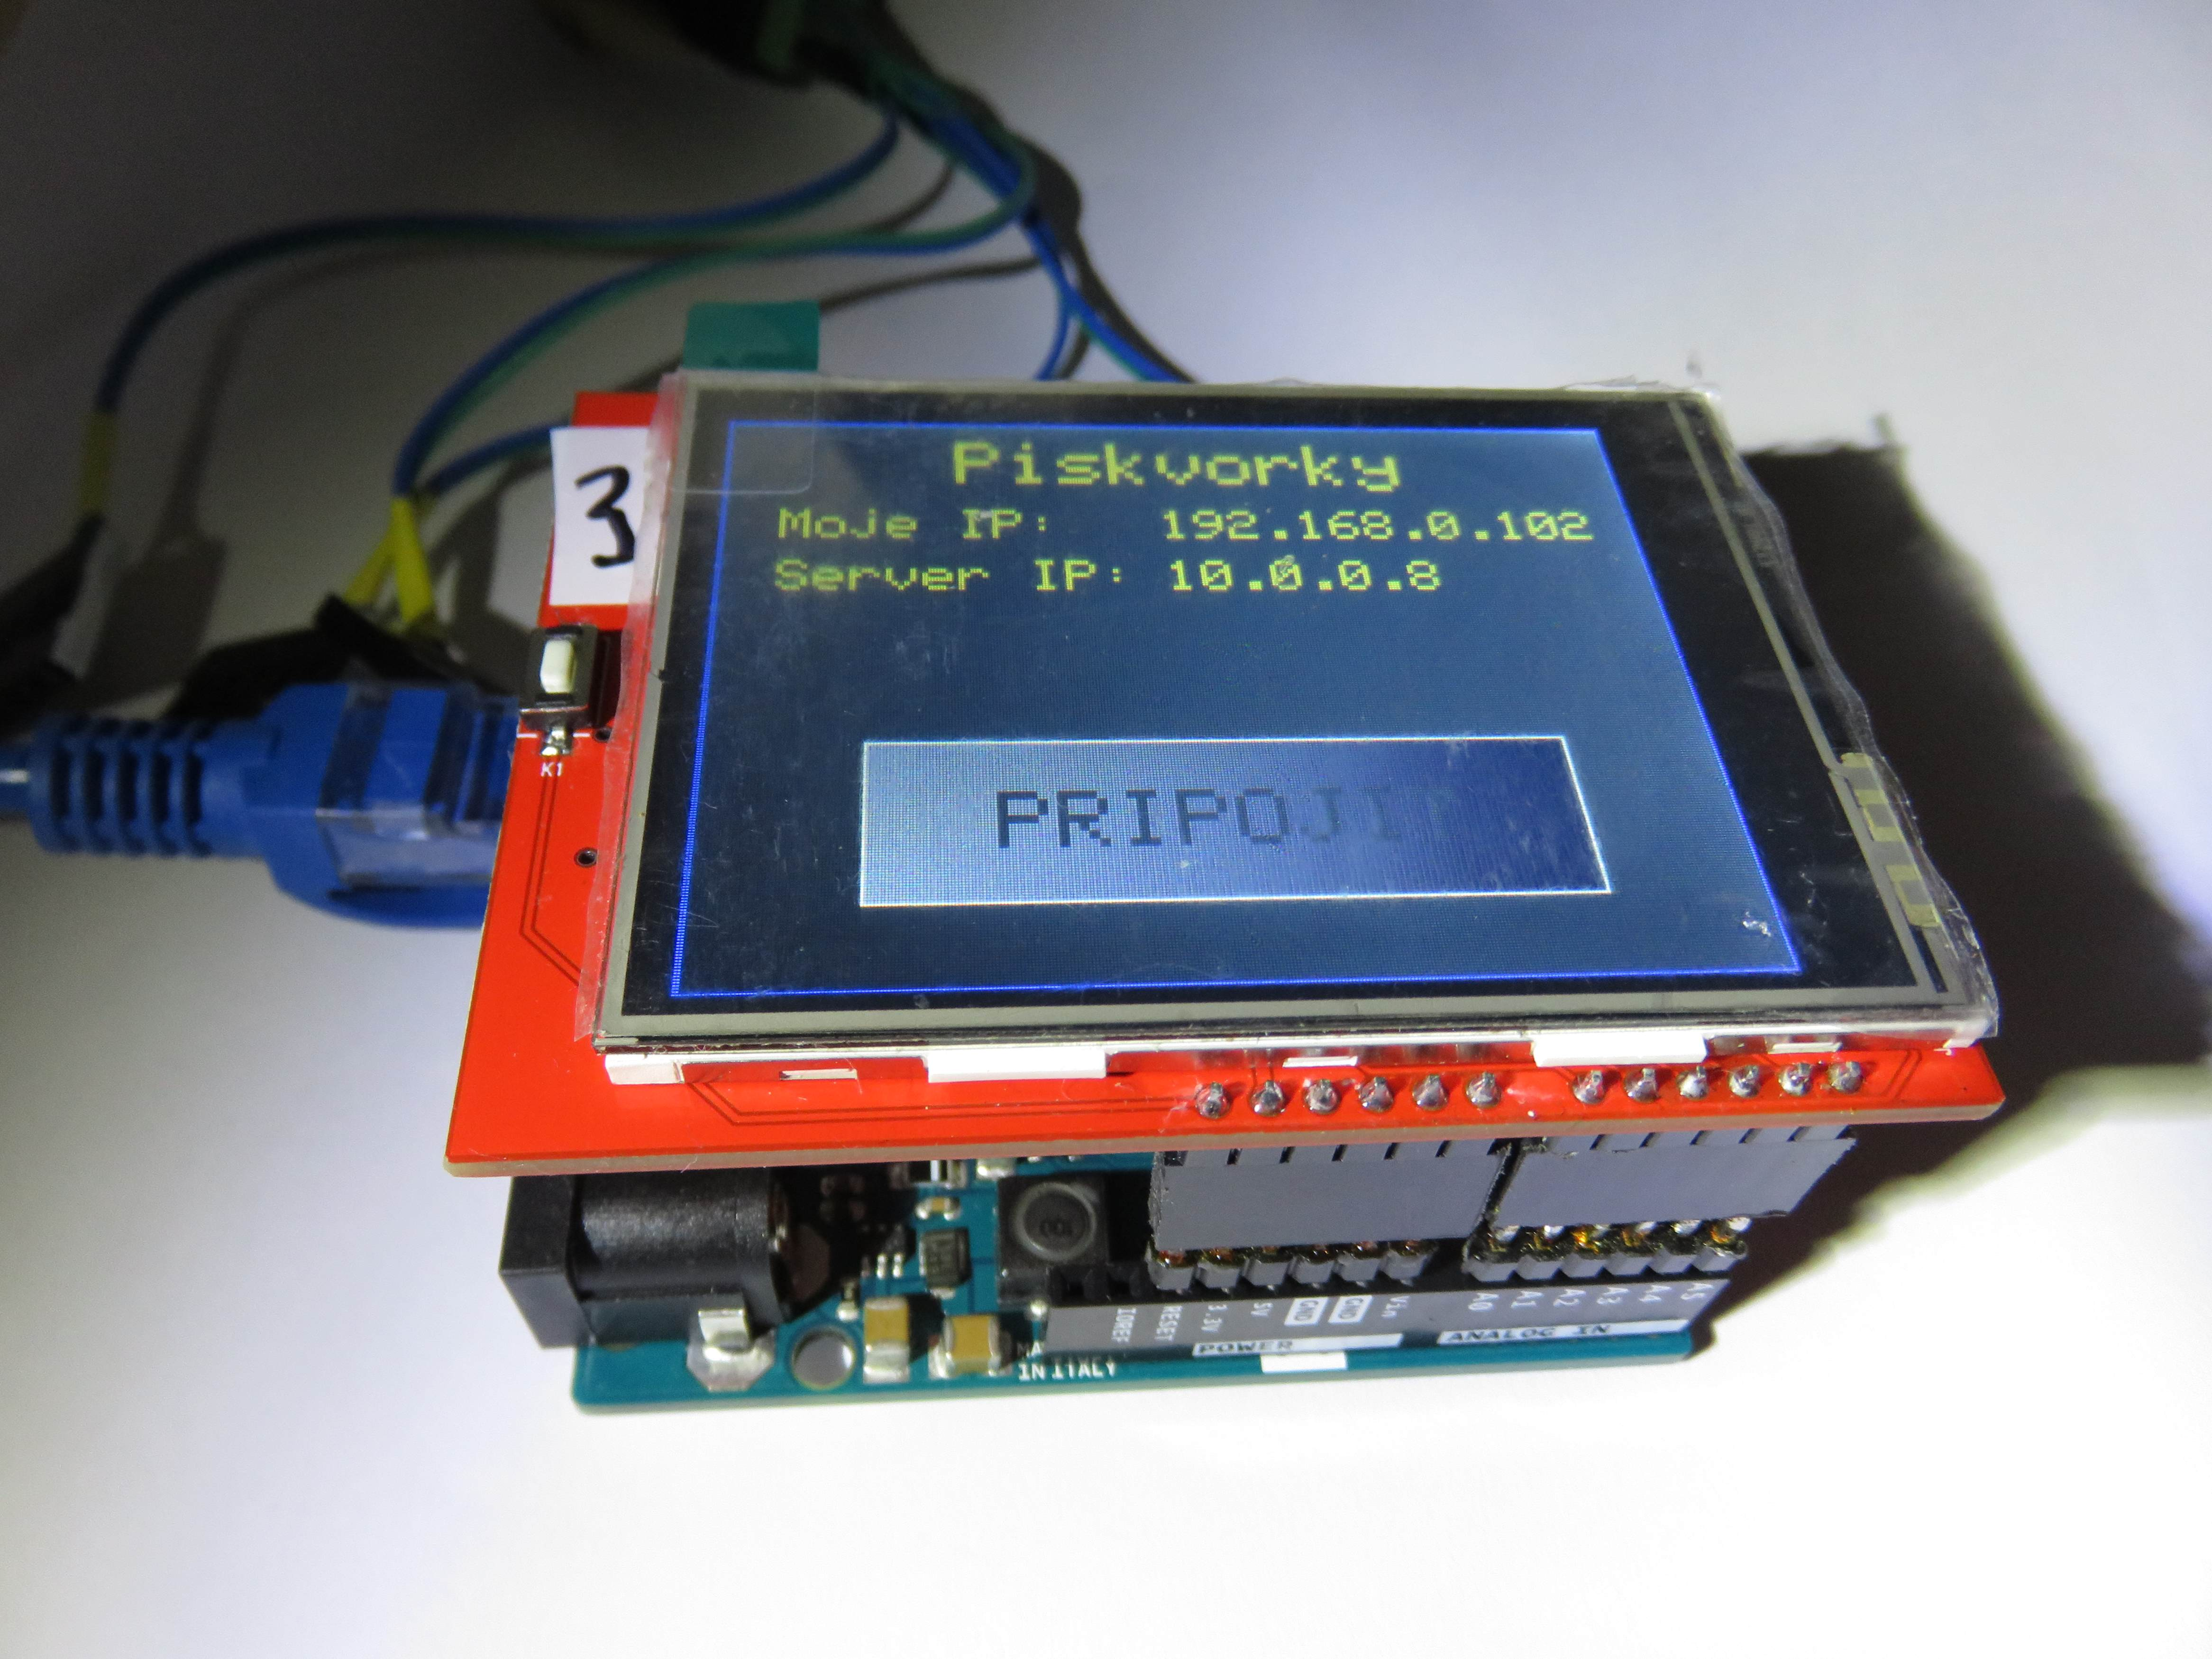
\includegraphics[width=10cm]{img/foto/HW_client.jpg}
\caption{\label{fig:HW_client} Fotografie funkční verze clienta}
\end{figure}
%_____________________________________

\subsection{Server}
\label{sec:server}
Základem serveru je Arduino Due (bližší specifikace v \cite{ArduinoDue_page}). Pro připojení do sítě byl zvolen Ethernetový shield s čipem Wiznet W5100. 

Pro pohodlné ovládání hry jsou k serveru připojena dvě tlačítka, tlačítko s červeným kroužkem slouží pro zastavení a restart hry, tlačítko se zeleným kroužkem slouží pro start hry. Schéma zapojení je vidět na obrázku \ref{fig:server_switch_module}. Zapojení bylo pro testovací účely zhotoveno na univerzální desce plošných spojů. Připojení je realizováno pomocí vodičů, kolíky umístěné v desce slouží pouze k připevnění k Arduinu nebo shieldu. Vodiče s připojí podle barvy následovně: 
\begin{enumerate}
\item Černý - GND
\item Modrý - D40
\item Oranžový - D38
\item Červený - 5 V
\end{enumerate}
Místo pinů D40 a D38 lze použít libovolné jiné, ale tato změna musí být upravena v kódu pro server (viz. kapitola \ref{sec:nastaveni_server}).
%Schéma modulu s tlačítky
\begin{figure}[hbtp]
\centering
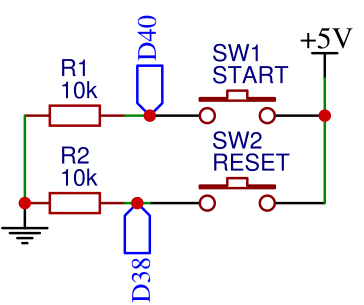
\includegraphics[width=5cm]{img/schema/server_switch_module.png}
\caption{\label{fig:server_switch_module}Schéma zapojení tlačítek pro ovládání serveru}
\end{figure}
%Fotografie serveru
\begin{figure}[hbtp]
\centering
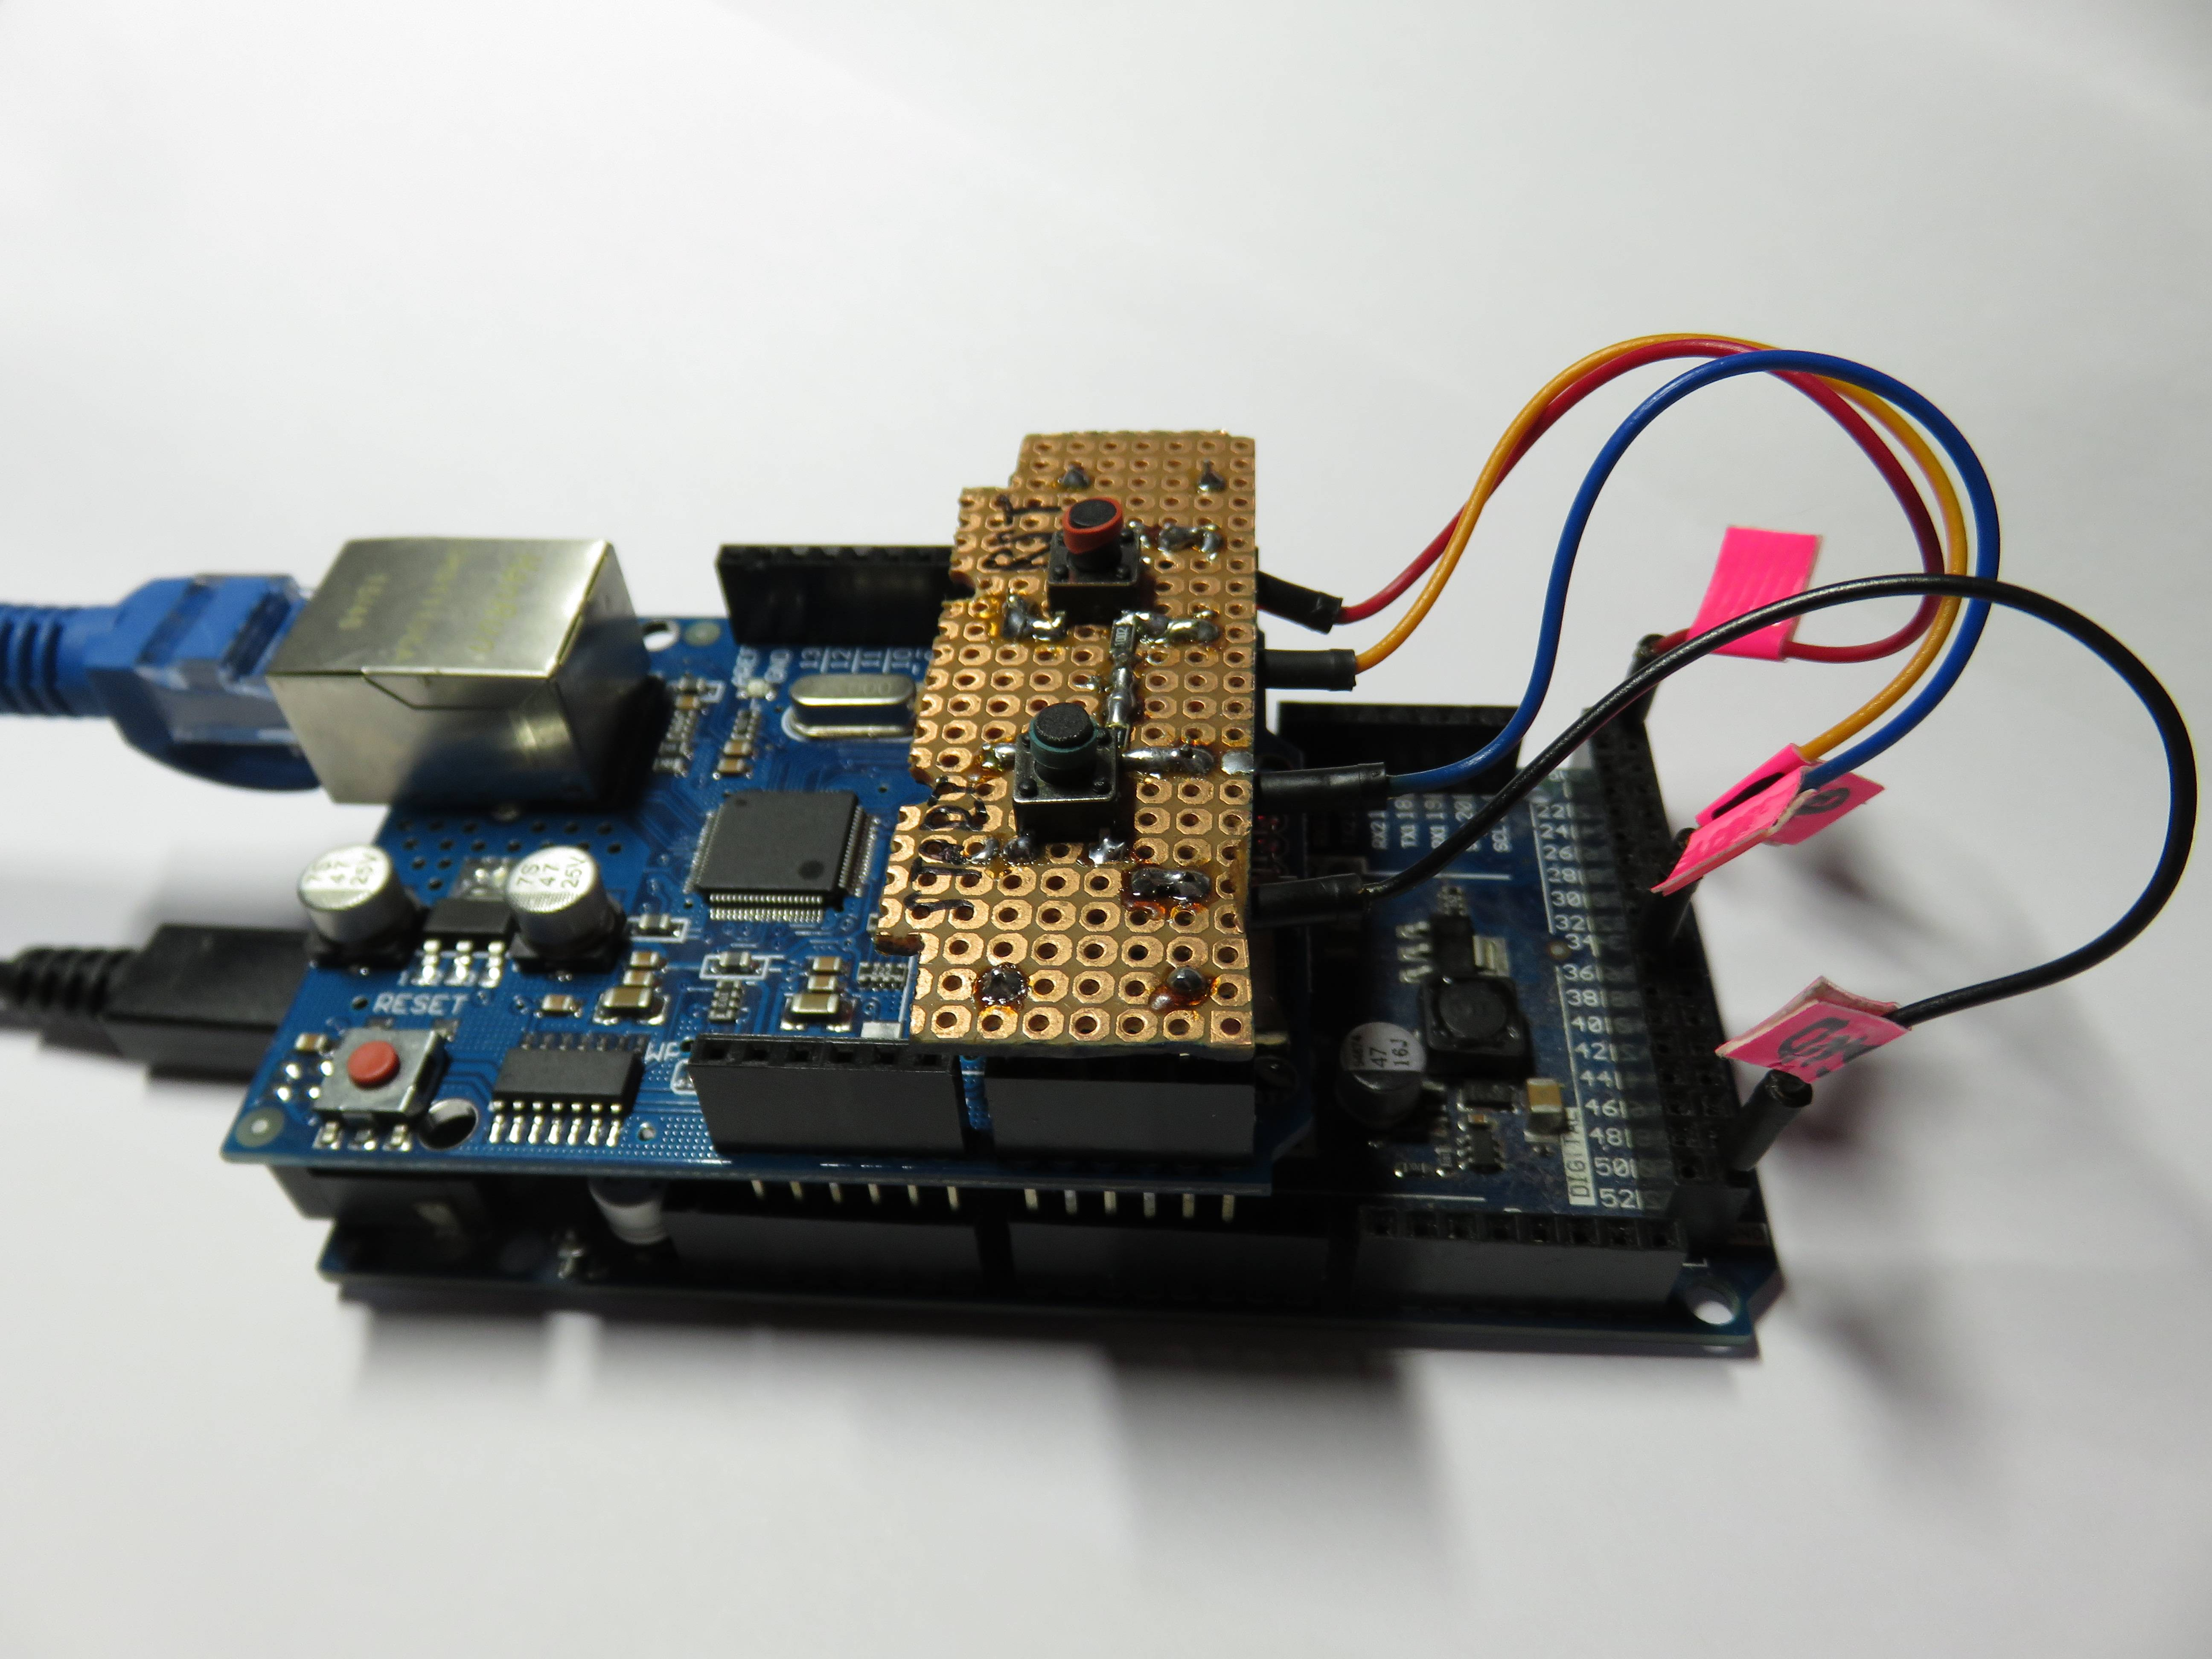
\includegraphics[width=10cm]{img/foto/HW_server.jpg}
\caption{\label{fig:HW_server}Fotografie funkční verze serveru}
\end{figure}
%____________________________________
\subsection{Napájení}
\label{sec:napajeni}
Napájení je řešeno externím zdrojem 5 V DC. Client se k napájení připojuje na programovací vstup (místo převodníku USB/UART), na piny: 1 = GND a 3 = 5V (zprava). Připojení externího zdroje pomocí souosého konektoru a využití integrovaného stabilizátoru není možné, protože client s displejem odebírá za provozu kolem 300 mA. 
%_____________________________________
\subsection{Router a nastavení sítě}
\label{sec:router}
Pro testování byl použit Huawei EchoLife HG520i. V nastavení byly vypnuty všechny funkce (WiFi apod.) a byl nakonfigurován DHCP server. Konfigurační soubor dostupný v příloze \ref{priloha:github_router_conf}.

Aby se Arduina mohla spojit, je nutná aby měl server statickou IP adresu. Tento router neumožňuje přiřazení IP adresy k dané MAC, proto má server pevně přiřazenou IP (její změna popsána v kapitole \ref{sec:nastaveni_server}). Tato adresa musí být ze stejné sítě jako je router ale mimo rozsah DHCP serveru.

Clientům je IP adresa přiřazována automaticky pomocí DHCP.
%_____________________________________
%=====================================
\clearpage
\section{Software}
%_____________________________________
\subsection{Knihovny}
\label{sec:knihovny}
Seznam použitých knihoven pro clienta:
\begin{itemize}
\item \textit{Ethernet library}: komunikace po LAN (se serverem), zdroj \cite{library_ethernet}.
\item \textit{UTFGLUE}: ovládání displeje, zdroj \cite{library_UTFGLUE}.
\item \textit{TouchScreen}: práce s dotykovou plochou, zdroj  \cite{library_touch}.
\end{itemize}

Seznam použitých knihoven pro server:
\begin{itemize}
\item \textit{Ethernet library}: komunikace po LAN (s jednotlivými clienty), zdroj \cite{library_ethernet}.
\end{itemize}
%_____________________________________
\subsection{Komunikace}
\subsubsection{Komunikace Server -> Client}
\label{sec:komunikace_server_client}
Během komunikace tímto směrem vždy server odešle celou herní desku (pole typu byte \textit{board}), celkem tedy 136 bajtů. Pokud client toto pole v pořádku přijme, dojde k jeho vyhodnocení a vykonání potřebných funkcí (překreslení displeje, vyžádání akce od uživatele, zobrazení hlášky). Hodnoty pole mění pouze server. Popis pole a co které hodnoty představují je vidět v tabulce \ref{tab:board_content}. 

Při odesílání je pole rozděleno do packetů. Každý packet obsahuje 8 bajtů pole \textit{board}, pořadové číslo packetu (aby client mohl pole zpětně sestavit) a dva bajty kontrolního součtu. 

Client průběžně přijímá jednotlivé části, pokud dorazí nějaká část chybná (nesedí kontrolní součet), client si může vyžádat od serveru znovuodeslání (realizace popsána v kapitole \ref{sec:komunikace_client_server}). Pokud client přijme všechny části, pole \textit{board} vyhodnotí.
%Tabulka herní desky (pole board)
\begin{table}[hbtp]
\catcode`\-=12
\caption{\label{tab:packet_server-client}Rozložení pole \textit{board} pro přenos dat a řízení hry mezi serverem a klientem}
\begin{tabular}{|c|c|l|}
\hline
Index   & Hodnoty     & \multicolumn{1}{c|}{Popis}                                      \\ \hline
0-89    &             & Každý index odpovídá jednomu čtverečku na herní desce piškvorek \\ \cline{2-3}
        & 0           & Pole je prázdné (neobsazené)                                    \\ \cline{2-3}
        & 1-5         & Obsazeno některým hráčem/klientem                               \\ \hline
90      &             & Přenos řídicí informace pomocí kódu                             \\ \cline{2-3}
        & 0           & nic nedělat                                                     \\ \cline{2-3}
        & 1           & Vše je OK, překreslit obrazovku                                 \\ \cline{2-3}
        & 3           & Příprava nové hry, zobrazit úvodní obrazovku                    \\ \cline{2-3}
        & 9           & Informace pro hráč odpojen, že bude odpojen                     \\ \cline{2-3}
        & 100         & Hra skončila remízou                                            \\ \cline{2-3}
        & 10x         & Hodnota podle hráče, který vyhrál: 101-105 ('x' je číslo hráče) \\ \cline{2-3}
        & 20x         & Problémy/odpojení s daného hráče: 201-205 ('x' je číslo hráče)  \\ \hline
91      & 1-5         & Číslo hráče, který je na tahu, pokud je 0, nikdo nehraje        \\ \hline
93      & 0-89        & Počet odehraných kol (vyplňuje server)                          \\ \hline
95-96   &             & Barva hráče 1                                                   \\ \cline{1-1} \cline{3-3}
97-98   &             & Barva hráče 2                                                   \\ \cline{1-1} \cline{3-3}
99-100  & Kód barvy   & Barva hráče 3                                                   \\ \cline{1-1} \cline{3-3}
101-102 &             & Barva hráče 4                                                   \\ \cline{1-1} \cline{3-3}
103-104 &             & Barva hráče 5                                                   \\ \hline
105-108 &             & IP adresa hráče 1                                               \\ \cline{1-1} \cline{3-3}
109-112 &             & IP adresa hráče 2                                               \\ \cline{1-1} \cline{3-3}
113-116 & IPv4 adresa & IP adresa hráče 3                                               \\ \cline{1-1} \cline{3-3}
117-120 &             & IP adresa hráče 4                                               \\ \cline{1-1} \cline{3-3}
121-124 &             & IP adresa hráče 5                                               \\ \hline
\end{tabular}
\end{table}

%
\subsubsection{Komunikace Client -> Server}
\label{sec:komunikace_client_server}
Při této komunikaci se přenáší vždy dva bajty, přičemž celá zpráva je odeslána dvakrát po sobě. Server po přijetí obou zpráv zprávy porovná a pokud se neliší provede dané instrukce (význam v tabulce XXX). V případě neshody je zpráva zahozena. 
%Tabulka přenášeného packetu
\begin{table}[hbtp]
\catcode`\-=12
\caption{\label{tab:clietn-server} Rozložení packetu pro komunikaci klient - server}
\begin{tabular}{|c|c|l|}
\hline
Index & Hodnoty                         & \multicolumn{1}{c|}{Popis}                                                                                                                                                                                \\ \hline
0     & 10                              & \begin{tabular}[c]{@{}l@{}}Jedná se o informaci, že další přenesený bajt bude číslo vyplněné\\ herní pozice v poli \textit{board}    \end{tabular} \\ \cline{2-3}
      & 20                              & \begin{tabular}[c]{@{}l@{}}Žádost klienta o poslání dané části herního pole (board), v další \\ bajtu je číslo dané části \textit{boardu}   \end{tabular}   \\ \hline
1     & \multicolumn{1}{l|}{0-89, 0-16} & \begin{tabular}[c]{@{}l@{}}Podle hodnoty předchozího bajtu: index vyplněného \\ pole nebo pořadí packetu, který má být poslán znovu\end{tabular}                                                          \\ \hline
\end{tabular}
\end{table}

%_____________________________________
\subsection{Změny a nastavení}
\subsubsection{Server}
\label{sec:nastaveni_server}

%_____________________________________
\clearpage
\section{Závěr}
%
%>>>>>>> Seznam literatury <<<<<<<
\clearpage
%--- Změna nadpisu literatury
\renewcommand{\refname}{Seznam použité literatury a zdrojů informací}
\addcontentsline{toc}{section}{Seznam použité literatury a zdrojů informací}
\begin{thebibliography}{99}
\bibitem{arduinoEthernet_page}
\textit{Arduino store: ARDUINO ETHERNET REV3} [online]. [cit. 2019-02-05]. Dostupné z: https://store.arduino.cc/arduino-ethernet-rev3-without-poe
%%%
\bibitem{library_ethernet}
\textit{Arduino: Ethernet library} [online]. [cit. 2018-12-18]. Dostupné z: https://www.arduino.cc/en/Reference/Ethernet
%%%
\bibitem{ArduinoDue_page}
\textit{Arduino store: ARDUINO DUE} [online]. [cit. 2019-02-05]. Dostupné z: https://store.arduino.cc/arduino-due
%%%
\bibitem{library_UTFGLUE}
MCUFRIEND\_kbv library. \textit{Github} [online]. [cit. 2019-02-05]. Dostupné z: https://github.com/prenticedavid/MCUFRIEND\_kbv
%%%
\bibitem{library_touch}
Adafruit\_TouchScreen library. \textit{Github} [online]. [cit. 2019-02-05]. Dostupné z: https://github.com/adafruit/Adafruit\_TouchScreen
\end{thebibliography}
%--- SEZNAM SOFTWARU ---
\clearpage
\phantomsection %pridej odkaz do PDF zalozek
\addcontentsline{toc}{section}{Seznam použitého softwaru}
\section*{Seznam použitého softwaru}
\begin{enumerate}%[--]
	\item \TeX maker, \TeX Live
	\item \href{https://www.arduino.cc/en/main/software}{Arduino IDE}
	\item \href{https://www.tablesgenerator.com/latex_tables}{Tables Generator}
	\item \href{https://www.citace.com/citace-pro}{Citace.com}
	\item \href{https://easyeda.com/}{EasyEDA}
	\item \href{https://www.irfanview.com/}{IrfanView}
	\item \href{https://linuxmint.com/}{Linux Mint 18.1 Cinnamon 64-bit}
\end{enumerate}
%--- SEZNAM PRILOH ---
\phantomsection %pridej odkaz do PDF zalozek
\addcontentsline{toc}{section}{Seznam příloh}
\section*{Seznam příloh} 
\begin{enumerate}[{Příloha} 1:]
\item \label{priloha:github_router_conf} Konfigurační soubor routeru Huawei EchoLife HG520i na Githubu, dostupné z: \href{https://goo.gl/h8494S}{https://goo.gl/h8494S}
\end{enumerate}
\end{document}